\chapter{Results}

This chapter presents the findings of the experiments conducted in this masters thesis. The chapter is divided into two sections.
The first section presents the results of\method{1}, the second section presents the results of \method{2},
 where both methods will be evaluated in context of both Gaussian VAEs and VQ-VAEs.

\section{Results of \method{1}}

In this section, I will present the results of \method{1} on both Gaussian VAEs and VQ-VAEs.

\subsection{Results on Gaussian VAEs}
% Think about: Coefficients, Number of pixels to be sampled. How it changes the results.
The experiments on Gaussian VAEs were run on multiple configurations of encoder and decoder architectuers. 
The expiremnts were run on both latent space of 16 and 64 dimensions. 


\begin{figure}[H]
    \centering
    \centering
\scriptsize
\begin{tabular}{||c|c|c|c||}
\hline
 Method & Parameters & Reconstruction loss & KL loss \\
\hline
\textit{Baseline} & - & 0.0042 +- 1.2e-03 & 0.0018 +- 6.3e-04 \\
\hline
Multi Decoder & Exact sampling & 0.0036 +- 8.3e-04  $\downarrow$ & 0.0027 +- 8.7e-04  $\uparrow$ \\
\hline
Multi Decoder & Exact sampling, SoftAdapt & 0.0034 +- 1.9e-04  $\downarrow$ & 0.0029 +- 2.8e-03  $\uparrow$ \\
\hline
Multi Decoder & Uniform sampling & 0.0035 +- 6.5e-04  $\downarrow$ & 0.0026 +- 1.7e-03  $\uparrow$ \\
\hline
Multi Decoder & Uniform sampling, SoftAdapt & 0.0034 +- 7.3e-03  $\downarrow$ & 0.0029 +- 2.0e-02  $\uparrow$ \\
\hline
\end{tabular}

    \caption[Trained neural network with \method{1} applied to a Gaussian VAE.]
    { Trained neural network with \method{1} applied to a Gaussian VAE on CelebA dataset and latent space 16.
    }
    \label{fig:res_val}
\end{figure}

\begin{figure}[H]
    \centering
    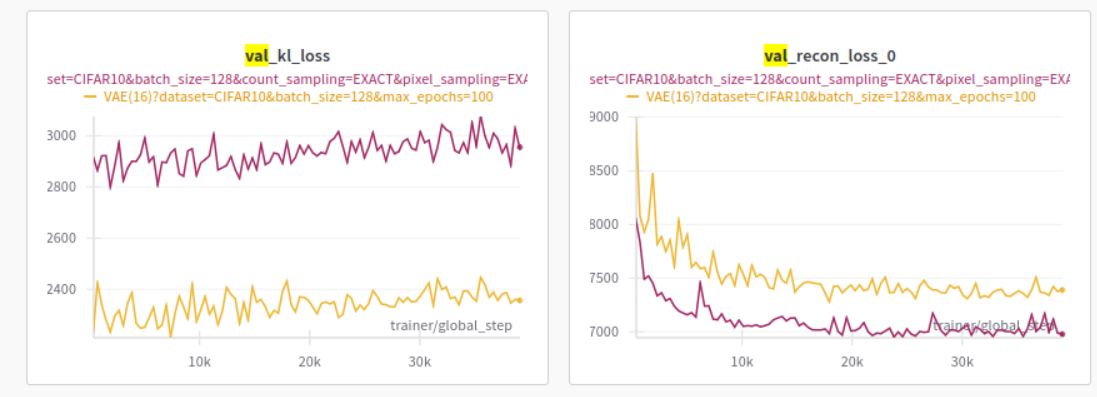
\includegraphics[width=0.8\textwidth]{figures/SCVAE2D_16_CIFAR10.png}
    \caption{KL divergence of the latent space of the Gaussian VAEs.}
    \label{fig:kl_divergence_gaussian_vae}
\end{figure}

\subsubsection{Exact same sampling}

\subsubsection{Uniform sampling}

\subsection{Results on VQ-VAEs}

\subsubsection{Exact same sampling}

\subsubsection{Uniform sampling}


\section{Results of \method{2}}

In this section, I will present the results of \method{2} on both Gaussian VAEs and VQ-VAEs.

\subsection{Results on Gaussian VAEs}

\subsubsection{Uniform random sampling}

\subsubsection{Gaussian sampling}

\subsection{Results on VQ-VAEs}

\subsubsection{Uniform random sampling}

\subsubsection{Gaussian sampling}


